\section{Capítulo 5: Algoritmos Distribuidos}
\subsection{Conceptos Básicos}

\textbf{Definición}: Tipo de algoritmo que se ejecuta concurrentemente en una red de procesos, con información limitada sobre los demás procesos. Trabajando cooperativamente mediante paso de mensajes en lograr un objetivo común.

Ejemplos: Ordenamiento de eventos, mensajes u operaciones. Observación o monitoreo consistente. Elección de un líder o coordinador. Exclusión mutua distribuida.

\textbf{Caracterización de algoritmos distribuidos}: \begin{itemize}
    \item Tipo de topología: Anilo, árbol, grafo general (dirigido o no dirigido, total o parcialmente conectado)
    \item Modelos de computación: Estilo de interacción, modelo de sincronismo y restricciones temporales, modelo de fallas y fiabilidad
    \item Medidas de desempeño: Complejidad de mensajes (\# mensajes), complejidad de tiempo (\# rondas)
    \item Técnicas de diseño: Números de secuencia, relojes lógicos o vectoriales, marcas de tiempo para mensajes, contadores de mensajes, métodos de asentimiento (acknowledge), métodos de crédito, paso de testigo (token-passing)
\end{itemize}

\subsection{\textbf{Algoritmo de Eco-Chang}}

\textbf{Objetivo}: Visitar paralelamente todos los nodos de una red de procesos, representada como una topología de grafo general no dirigido, generando un spanning tree.

\textbf{Requisitos}: Topología de grafo general no dirigido y conexo. Se asume para el sistema o red de procesos un modelo asincrónico y sin fallas. Comunicación entre procesos es por paso de mensajes asincrónico y bidireccional. Cada nodo sólo conoce a los vecinos con quienes está directamente conectado. Existe un único nodo que comienza el algoritmo \textbf{(nodo iniciador)}

\textbf{\textcolor{blue}{Algoritmo de dos fases}}: \begin{itemize}
    \item \textbf{Exploración}: El nodo iniciador envía un mensaje a todos los nosdos de la red.
    \item \textbf{Eco}: Asentimiento (acknowledge) de los nodos que recibieron el mensaje, mandando un eco de vuelta al nodo iniciador.
\end{itemize}

\textbf{\textcolor{blue}{Comportamiento básico}}: \begin{itemize}
    \item Nodo \textbf{iniciador} envía el mensaje de \textbf{exploración} a sus vecinos.
    \item Si un nodo recibe el mensaje por primera vez, este \underline{memoriza el vecino de origen} y distribuye el mensaje a sus otros vecinos.
    \item Un nodo solo envía el mensaje de \textbf{eco} al vecino de origen cuando ha recibido mensajes de eco de todos sus otros vecinos.
    \item El algoritmo termina cuando el nodo iniciador recibe un mensaje de \textbf{eco} de todos sus vecinos.
\end{itemize}

\textbf{{\textcolor{purple}{Variables del algoritmo en cada proceso}}}: \begin{itemize}
    \item \textbf{comprometido}: Booleano que indica si está actibo el algoritmo en el proceso.
    \item \textbf{iniciador}: Booleano que indica si el proceso es iniciador.
    \item \textbf{n}: contador que indica número de mensajes recibidos por el proceso desde sus vecinos.
    \item \textbf{origen}: identifica al vecino desde el cual le llegó al proceso el \underline{primer} mensaje de exploración.
\end{itemize}

\textbf{Observación}: Inicialmente se asume que todo nodo no es iniciador, que no están comprometidos y que no han recibido mensajes.

\textbf{Observación 2}: Si el Eco de Chang se inicia varias veces en una misma topologia por nodos distintos., lo que se genera se denomina como \textcolor{red}{\textbf{bosque}}, vale decir tambien, que cada iniciador tiene un arbol distinto.
\vspace{0.5em}

\textbf{Observación 3}: Aun con ciclos, este algoritmo converge.

\textbf{Observación 4}: El como se genera el arbol depende de la velocidad de transmisión del explorador entre nodos 
\textbf{Complejidad}: \textcolor{red}{\textbf{Tiene complejidad 2e mensajes}}, donde \textbf{e} es el número de aristas del grafo

Se usa paso de mensajes unidireccional y asincrónico. El algoritmo genera un spanning tree. Tiene aplicación para recolectar y difundir información ordenadamente en un grafo general. Se supone que el algoritmo se \underline{se inicia sólo en un nodo}.

\subsection{Algoritmos de elección}
\textbf{Objetivo}: Ponerse de acuerdo en una red de procesos, suponiendo que los procesos están únicamente identificados y es posible ordenarlos totalmente.

Ejemplos: Determinación de un único coordinador o líder para un grupo de procesos cooperativos. Elección de un coordinador para gestionar una transacción distribuida y comprometerla, etc.

Existe la posibilidad de que se pregunte el nuevo coordiandor antes de tiempo, si pasa esto, puede existir dos coordinadores \textcolor{red}{\textbf{(Cortar el algoritmmo antes de tiempo)}}.
\vspace{0.5em}

\textbf{Caracterización} \begin{itemize}
    \item \textbf{Topología}: Anillo, árbol, red totalmente conectada, grafo general (arbitrario).
    \item \textbf{Modelo del sistema}: Asincrónico vs Sincrónico, modelo de fallas
    \item \textbf{Criterios típicos de diseño}: Nodos o procesos con identificador único, usado como criterio de selección. Principio de extinción de mensajes para garantizar término del algoritmo en tiempo finito. Simetría: nodos iguales que ejecutan el mismo algoritmo y cualquiera es elegible. Nodos tienen conocimiento sólo de sus vecinos.
\end{itemize}

\subsubsection{Elección en un grafo general}

\textbf{Claves de diseño del algoritmo}: Modelo asincrónico, con paso de mensajes unidireccional y fiable. Se elige como líder al proceso con mayor identificador del sistema. Propagar identificador máximo conocido por un nodo. Identificadores menores se extignuen y dejar de propagarse, al ser dominador por algún máximo relativo. Sólo \textbf{mayor identificador logra propagarse} y alcanzar a todos los nodos de la red. Sólo procesos candidatos en una elección ejecutan la partida del algoritmo.

\begin{figure}[H]
    \centering
    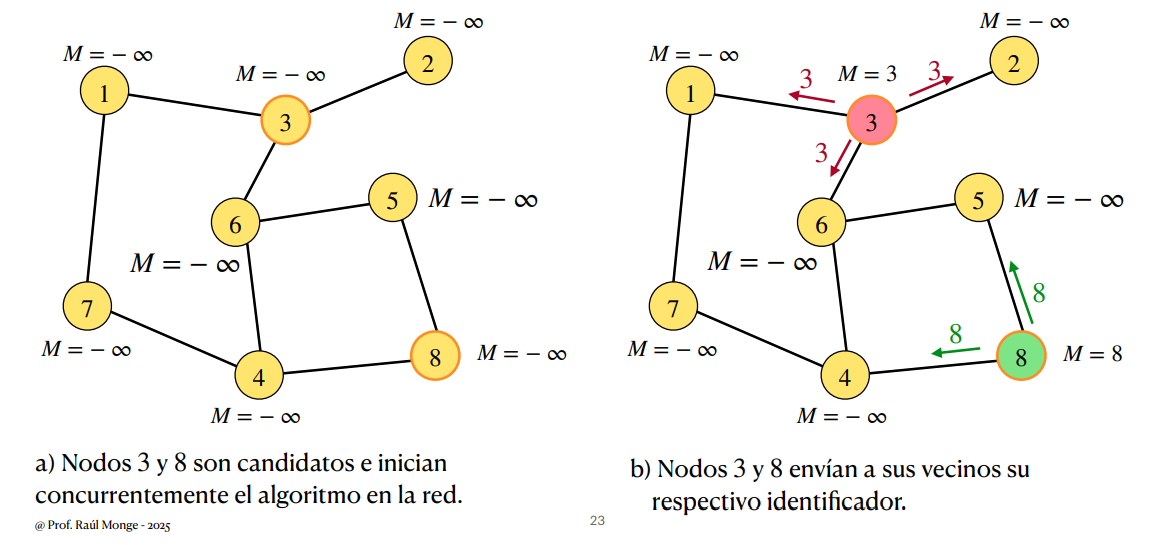
\includegraphics[width=0.25\textwidth]{img/GG_1.png}
    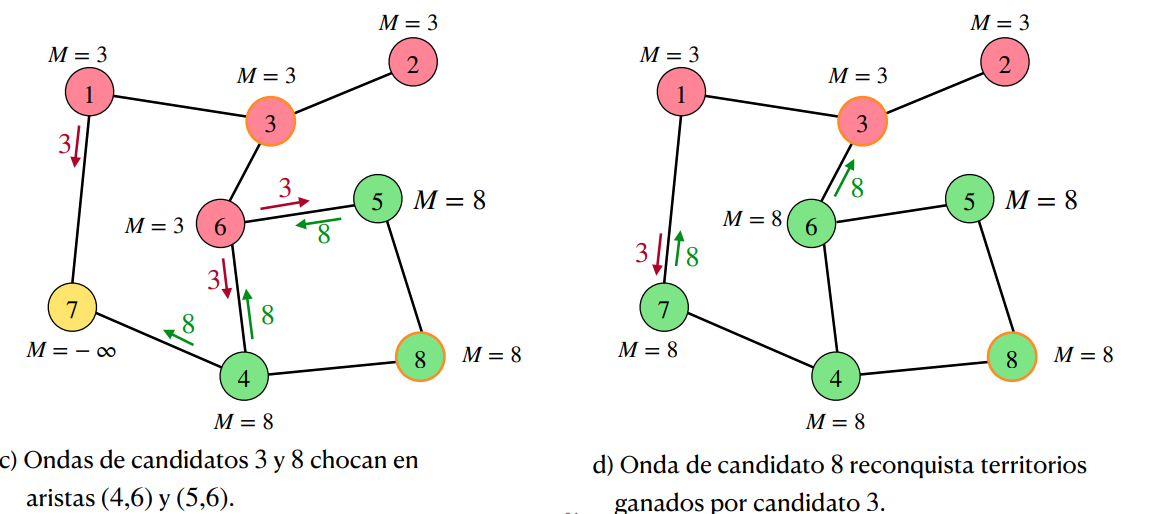
\includegraphics[width=0.25\textwidth]{img/GG_2.png}
    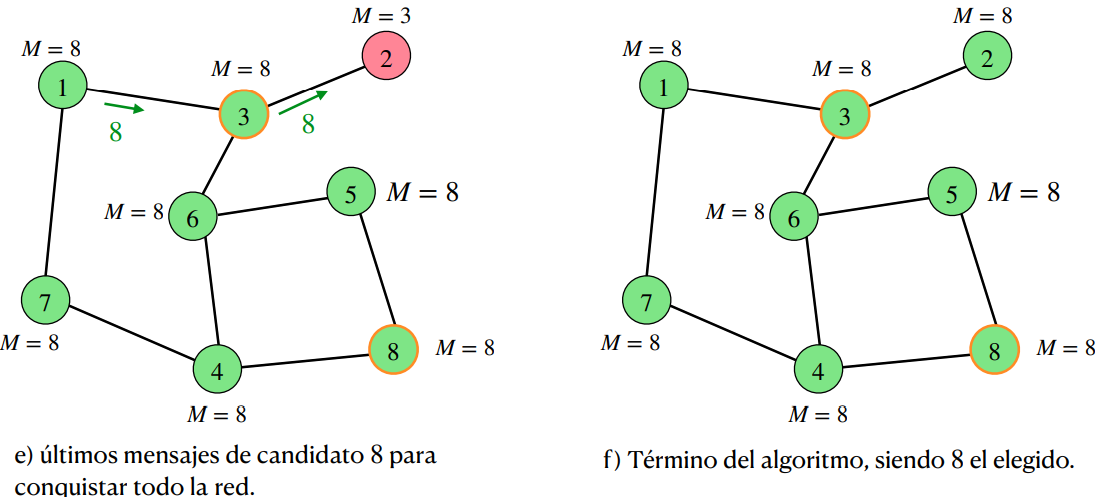
\includegraphics[width=0.25\textwidth]{img/GG_3.png}
    \caption{Esquema de elección en un grafo general}
\end{figure}

\subsubsection{Elección en un anillo unidireccional} 

\textbf{Claves de diseño del algoritmo}: Es similar al anterior, pero permite una elección en una topología de anillo unidireccional. Modelo asincrónico, con paso de mensajes unidireccional y fiable. Se elige como líder al proceso con mayor identificador. Sólo mayor identificador logra circular por todo el anillo. Usado en redes token-ring.

\textbf{Comentarios}: Mensajes con identificador menor que M se extinguen. Si un iniciador le llega un mensaje de elección con su propio identificador, entonces toma conocimiento que ha sido elegido. El algoritmmo se puede extender, para que en una segunda ronda el ganador comunique a los otros nodos que ha sido elegido.

\begin{figure}[H]
    \centering
    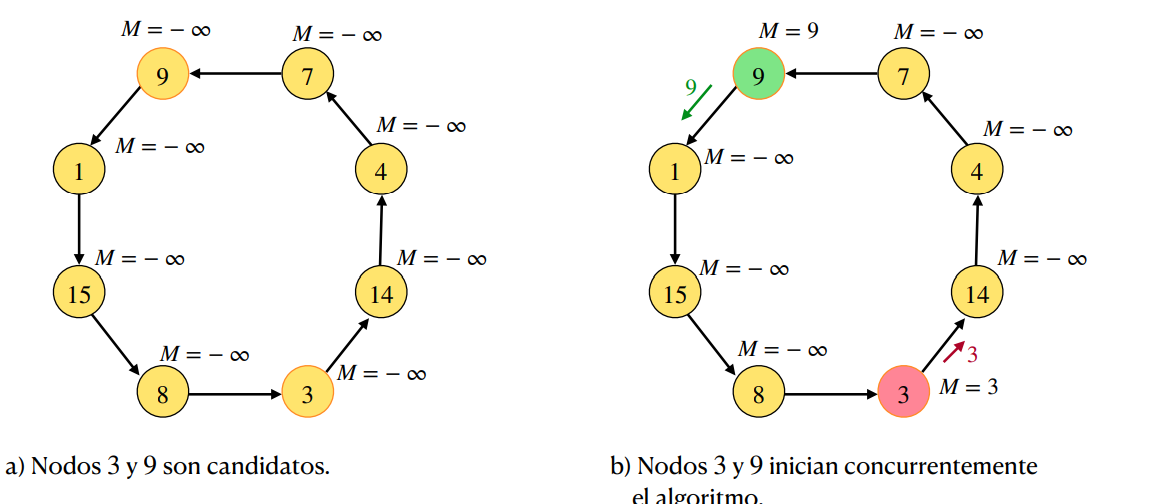
\includegraphics[width=0.25\textwidth]{img/AU_1.png}
    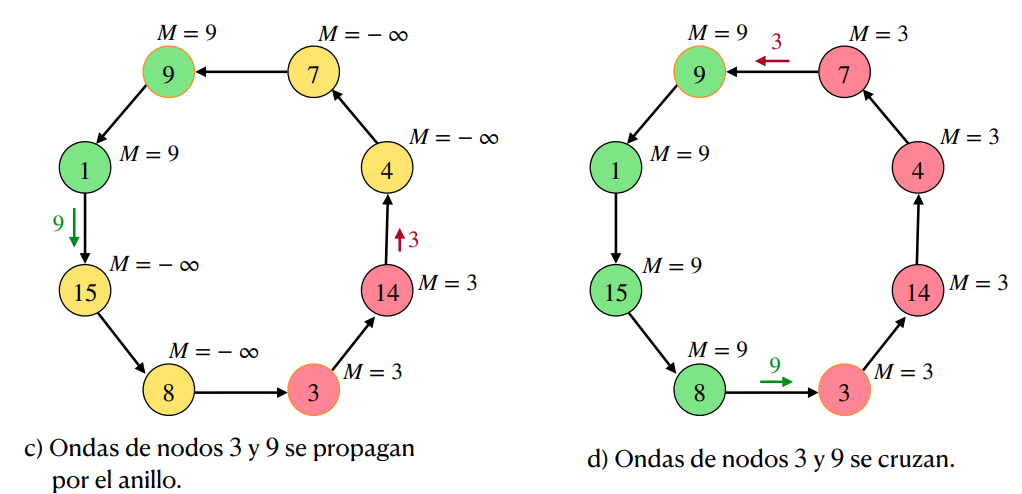
\includegraphics[width=0.25\textwidth]{img/AU_2.png}
    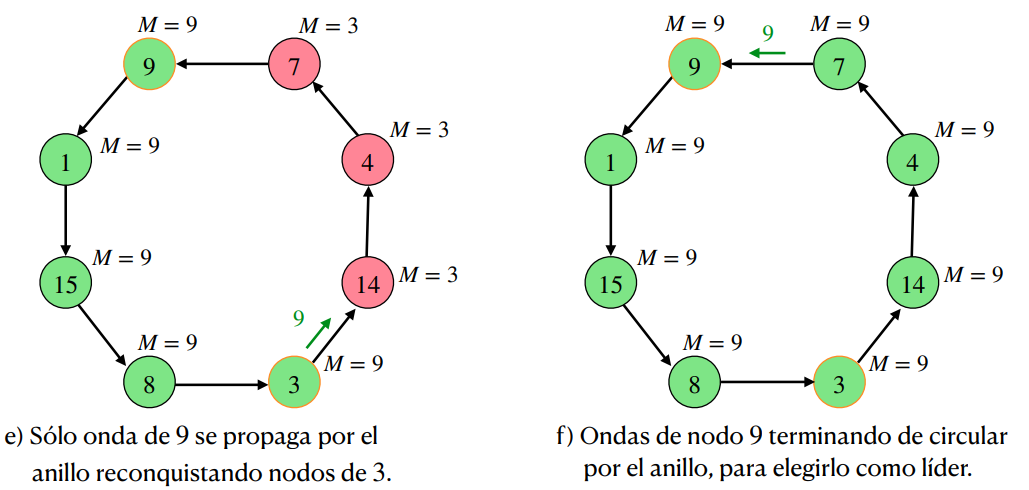
\includegraphics[width=0.25\textwidth]{img/AU_3.png}
    \caption{Esquema de elección en un anillo unidireccional}
\end{figure}

\subsubsection{Elección en un grafo totalmente conectado con fallas de proceso}

\textbf{Algoritmo del matón}:

\begin{itemize}
    \item \textbf{Requisito de conectividad}: Cada proceso conoce a todos los demás y existe conectividad completa. Cualquier nodo se comunica con un \underline{broadcast} con todos y fiablemente.

    \item \textbf{Inicio del algoritmo}: Se inicia cuando un proceso diferente al coordinador detecta que éste ha fallado, lo que puede ocurrir \underline{concurrentemente} en varios procesos. Corresponde a un mecanismo de \underline{heartbeat}, donde el coordinador manda periódicamente un mensaje avisando que \textcolor{blue}{está vivo}. La detección requiere uso de \underline{timers}, por lo tanto usa un modelo \textbf{sincrónico}.

    \item \textbf{Lógico del algoritmo}: Cada proceso envía un mensaje de control especial sólo a procesos con \textcolor{red}{mayor identificador}, estos procesos reciben el mensaje y responde con OK solo a procesos con \textcolor{red}{menor identificador}. Proceso que no recibe respuesta, se hace coordinador y lo comunica a los demás, si recibe respuesta de uno \textcolor{red}{mayor abandona} la elección.
\end{itemize}

\textbf{Comentarios}: Se requiere una red de conexión directa entre cualquier par de nodos. Cada nodo requiere conocer a todos los demás y como se ordenan. Opera en un modelo sincrónico. Es necesario disponer de un cierto nivel de sincronismo, para saber hasta cuánto esperar. Para detectar la falla del coordinador se usan algoritmos de tipo \underline{heartbeat}

\begin{figure}[H]
    \centering
    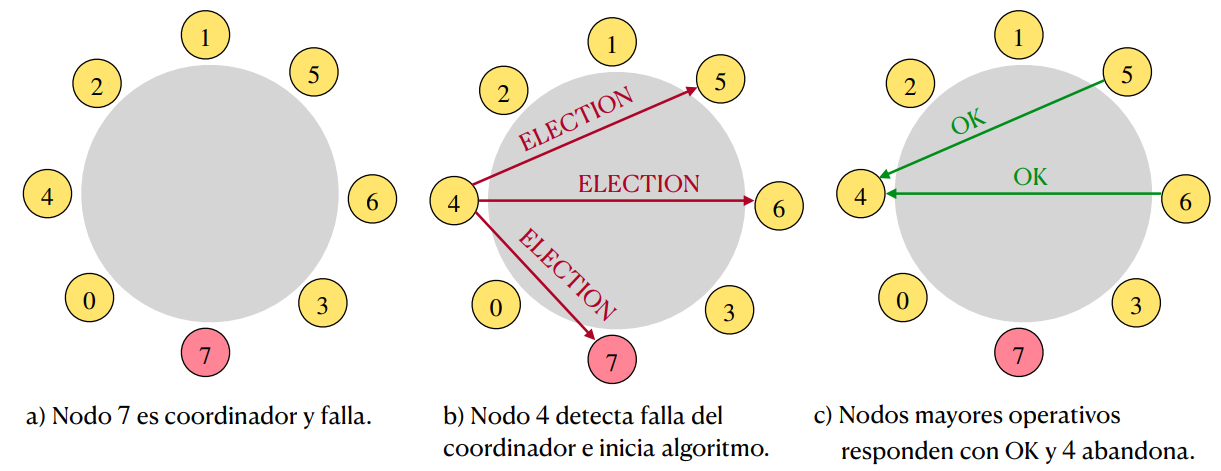
\includegraphics[width=0.25\textwidth]{img/Bully_1.png}
    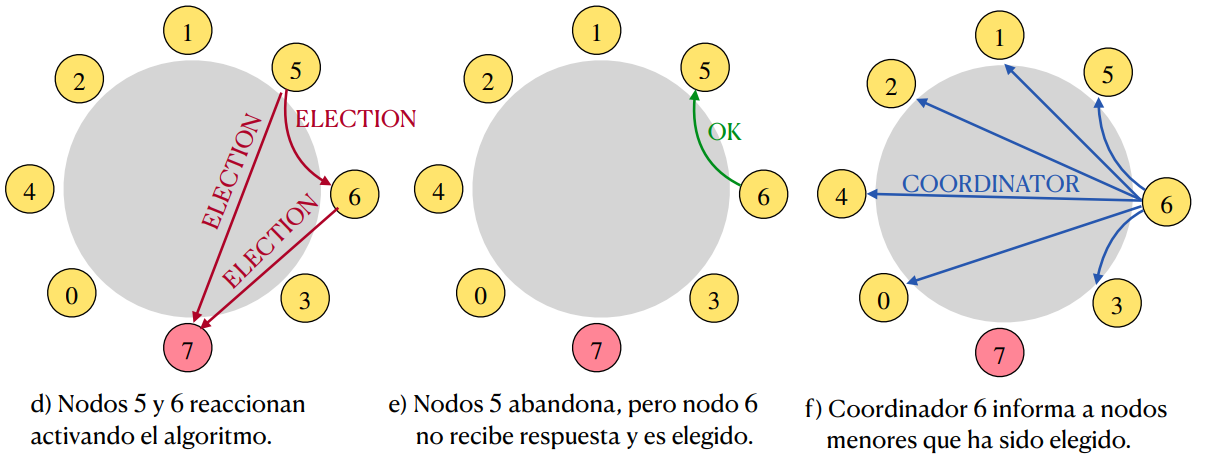
\includegraphics[width=0.25\textwidth]{img/Bully_2.png}
    \caption{Esquema del algoritmo del matón}
    
\end{figure}

\subsection{Algoritmos distribuidos de exclusión mutua}

\textbf{Objetivo}: Garantizar que a lo más un único proceso puede ejecutar simultáneamente una sección crítica. Se requiere evitar condiciones de carrera, como coordinar acceso a un recurso, garantizar la consistencia de los datos o mantener el correcto funcionamiento de un sistema distribuido.

\begin{figure}[H]
    \centering
    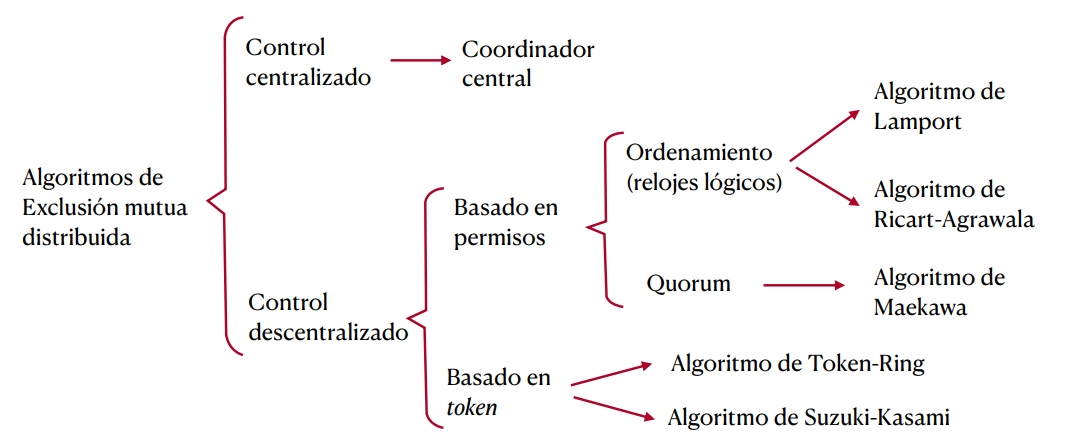
\includegraphics[width=0.25\textwidth]{img/Clasificacion_algoritmos.png}
    \caption{Esquema de exclusión mutua distribuida}
\end{figure}

\textbf{Una solución correcta para el problema de la exclusión mutua considera los siguientes estados y requisitos}

\begin{itemize}
    \item[a)] Estados de un proceso:
    
    $P_i$ respecto a la SC: \textbf{Requesting}: $P_i$ está solicitando ingresar a la SC; y se bloque si SC está ocupada por otro proceso. \textbf{Executing}: $P_i$ está ejecutando la SC y ningún otro proceso puede estar simultáneamente en este estado. \textbf{Idle}: $P_i$ esstá fuera de la SC, ejecutando acciones independientes; se dice que el proceso está ocioso.

    \item[b)] Requisitos para la solución:
    
    \textcolor{blue}{Seguridad}: En todo momento a lo más un proceso está en la SC. \textcolor{blue}{Vivacidad}: La solicitud a entrar en la SC se resuelve en tiempo finito. \textcolor{blue}{Justicia}: Si una sollicitud de ingreso a la SC sucede antes que otra, entonces la entrada a la SC es en ese orden.
\end{itemize}

Eventualmente podrán agregarse requisitos de rendimiento y resistencia a fallas.

\subsubsection{Exclusión mutua con control centralizado}

\textbf{Caracterización}: Requiere de un único proceso controlador que otorga el permiso para entrar a la SC. Procesos que solicitan permiso al controlador deben esperar respuesta para ingresar a su SC. La solución requiere 3 tipos de mensajes: 

\begin{itemize}
    \item \textcolor{blue}{Request}: Proceso solicita permiso a controlador para ingresar a su SC.
    \item \textcolor{blue}{Grant}: Controlador concede el permiso.
    \item \textcolor{blue}{Release}: Proceso que sale de su SC, avisa al controlador sobre su liberación.
\end{itemize}

\begin{figure}[H]
    \centering
    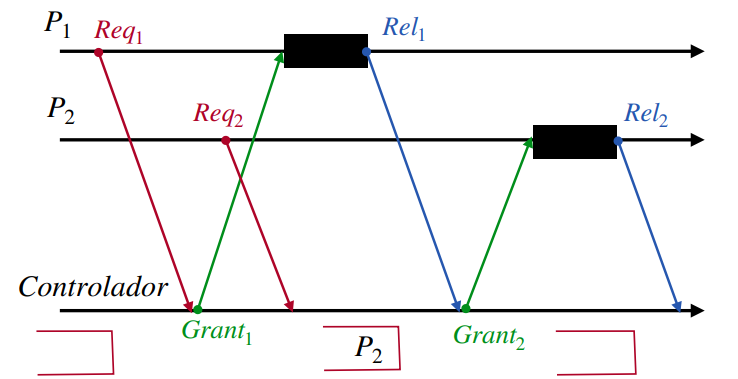
\includegraphics[width=0.25\textwidth]{img/E_M_Control_Centralizado.png}
    \caption{Esquema de exclusión mutua con control centralizado}
\end{figure}

\subsubsection{Algoritmos basados en token}

\begin{figure}[H]
    \centering
    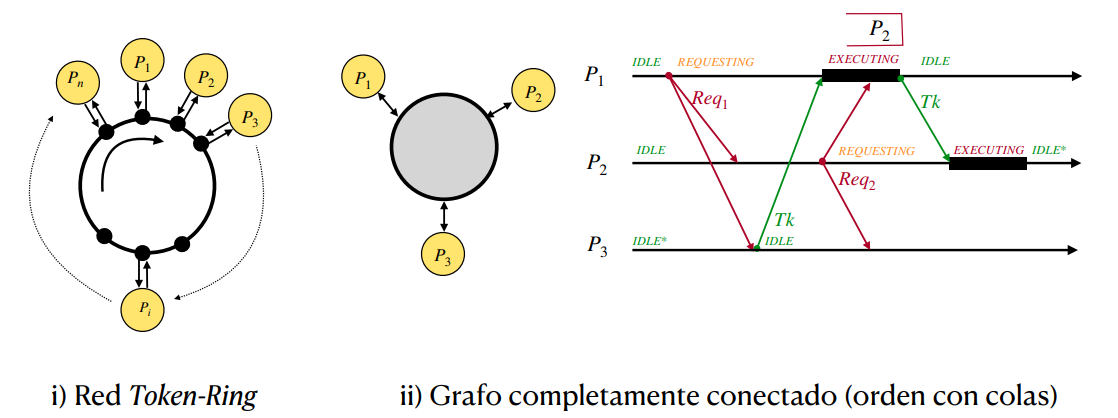
\includegraphics[width=0.25\textwidth]{img/Algoritmos_token.png}
    \caption{Esquema de algoritmo basado en token}
\end{figure}

\subsection{Algoritmo de Lamport} 

\textbf{Caracterización}: Algoritmo descentralizado basado en permisos, para un sisema asincrónico y basado en relojes lógico de lamport, para ordenar las solicitudes de ingreso a la SC.

\vspace{0.5em}
\underline{Condiciones para cada proceso $P_i$}: 

Mantiene un reloj lógico LC y marca sus solicitudes con el par $(TS_i, i)$, para estableceer un orden global único. 

Comunicación es por paso de mensajes asincrónico y garantiza orden FIFO para entrega de los mensajes. 

Mantiene cola \textcolor{blue}{$RequestQueue_i$} con solicitudes ordenadas ascendentemente por marca de tiempo. $R_i = \{P_1, P_2, \ldots, P_n\} : \forall i, 1 \leq i \leq n$

\vspace{0.5em}

\underline{Tipos de mensajes}: Request, Reply, Release.

\begin{figure}[H]
    \centering
    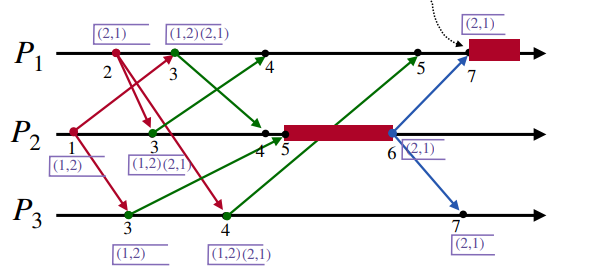
\includegraphics[width=0.25\textwidth]{img/A_Lamport.png}
    \caption{Esquema del algoritmo de Lamport}
\end{figure}

\textbf{Desempeño}: \textcolor{red}{3(N-1)} mensajes por cada invocación a la \textbf{SC}. \textcolor{magenta}{Retardo de sincronización: T. Throughput = $\frac{1}{E+T}$}

\textbf{Correctitud}: Es imposible que dos procesos vean en primera posición su solicitud en la cola, si sus canales son FIFO. Vivacidad y justicia son garantizadas por el orden de las solicitudes y el procesamiento en orden creciente de las marcas.

\subsection{Algoritmo de Ricart y Agrawala}

\textbf{Claves de diseño}: Comparte la misma caracterización general con el algoritmo de Lamport. Cada proceso requiere permiso de todos los demás procesos. Inicialmente se cumple \textcolor{blue}{$\forall i, 1 \leq i \leq n$: $State_i$ = IDLE $\wedge$ $RequestQueue_i$ = $\emptyset$}. La RequestQueue contiene a los procesos que han sido diferidos en el ingreso a la SC. Solo se requiere 2 tipos de mensajes: Request y Reply

Algo en tener en cuenta, con Ricart-Agrawala es que, el Reply (Verde en la siguiente figura) hace el trabanjo de Grant (para notificar el proximo proceso que tenga acceso a la SC), eso lo hace retrasando en envio de \textcolor{darkgreen}{\textbf{reply}} hasta el final.
\begin{figure}[H]
    \centering
    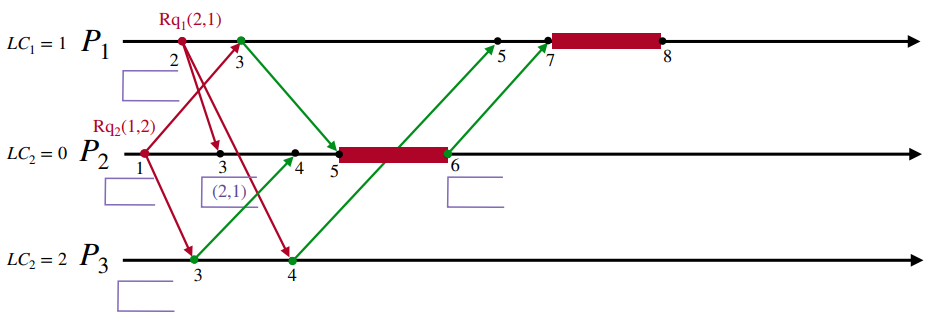
\includegraphics[width=0.33\textwidth]{img/A_Ricart_Agrawala.png}
    \caption{Esquema del algoritmo de Ricart y Agrawala}
\end{figure}

\textbf{Desempeño}: \textcolor{red}{2(N-1)} mensajes por cada invocación a la \textbf{SC}.  \textcolor{magenta}{Retardo de sincronización: T. Throughput = $\frac{1}{E+T}$}

\textbf{Correctitud}: Es imposible que dos procesos diferentes, si sus canales son FIFO, reciban un mensaje \textcolor{red}{REPLY} de los demás. Necesariamente el mayor de los dos va a ser diferido en la cola de menor marca. Vivacidad y justicia son garantizadas por el orden de las solicitudes y el procesamiento en orden creciente de las marcas.

\subsection{Algoritmo de Susuki-Kasami}

\textbf{Caracterización}: Algoritmo \textcolor{blue}{descentralizado basado en token}, para un sistema \textcolor{magenta}{asincrónico}. Garantiza \textcolor{magenta}{seguridad, vivacidad y justicia}.

\textbf{Características específica}: Un único token circula entre los procesos que lo solicitan y únicamente el proceso en posición del token puede hacer uso de SC, \textcolor{blue}{garantizando exclusión mutua}. Reduce la sobrecarga de mensajes; sin embargo, la pérdida del token interrumpe operación del sistema, lo que \textcolor{red}{requiere mecanismos de recuperación.}

\subsubsection{Idea general de funcionamiento}

Supondremos N procesos. Un proceso $P_i = (\forall i, 1 \leq i \leq N)$ que intenta regresar a la SC y que no tiene token, debe solicitarlo a los demás procesos. Difunde un mensaje REQUEST por el token a todos los demás procesos. El proceso que posee el token al recibir mensaje REQUEST, se lo envía al solicitante bajo las siguientes condiciones: 
\begin{itemize}
    \item El token se envía al solicitante sólo si el proceso en posesión de éste no está enla SC
    \item Si el proceso con el token estuviera en su SC, debiera retardar su envío hasta que salga de la SC.
    \item En el caso de existir varias solicitudes pendientes, se prioriza acceso que primero generó la solicitud.
\end{itemize}

El \textbf{token} es una estructura de datos que lleva  vector de registro de las solicitudes procesadas para cada proceso y mantiene una cola de solicitudes pendientes, estableciendo un orden de procesamiento y garantizando justicia y vivacidad.

\subsubsection{Claves de diseño}
\begin{itemize}
    \item[a)] \textbf{Identificador único de solicitudes}: Cada solicitud de un proceso $P_i$ se identifica con su UID y un número de secuencia $ns_i$ independiente de otros procesos. Luego, cada mensaje de solicitud queda únicamente identificada como: $REQUEST(i, ns_i)$
    \item[b)] \textbf{Arreglo de solicitudes por proceso}: $P_i$ mantiene $RN_i[1\ldots N]$, donde $RN_i[j]$ es la mayor solicitud recibida por $P_i$ desde $P_j$. Permite distinguir en el sistema entre solicitudes a\~{n}ejas y solicitudes recientes de un mismo proceso.
    \item[c)] \textbf{Token}: Es único en el sistema y consiste de una \textcolor{blue}{cola $Q$} y un arreglo de solicitudes completamente procesadas $LN[1 \ldots N]$. \textcolor{blue}{$Q$} corresponde a una cola FIFO que \underline{ordena} el ingreso a la SC de procesos que solicitan necesitan el token.  $LN[1 \ldots N]$ es un arreglo, donde $LN[i]$ contiene $ns_i$ de última solicitud procesada para proceso $P_i$  permite determinar qué procesos tienen solicitudes pendientes.
    \item[d)] \textbf{Lógica de procesos}: Un proceso $P_i$ en posición del token al salir de su SC, lo actualiza antes de considerar su envío haciendo: $P_i$ actualiza en el token: $LN[i] = RN[i]$. \textbf{Si} $RN_i[j] = LN[j] + 1$ y $P_j$ no está en la cola, \textbf{entonces} \textcolor{red}{$P_j$ tiene una solicitud pendiente y debe ser agregado }a $Q$
\end{itemize}

\textbf{Desempeño}: \textcolor{magenta}{Genera 0 a N mensajes por solicitud procesada, tiempo de sincronización: 0 o T, Throughput máximo = $\frac{1}{E+T}$}

El orden de agregar las solicitudes pendientes a la cola FIFO del token, es normalmente por nuevas solicitudes \textcolor{blue}{ordenadas por el identificador de proceso}. \textcolor{red}{El orden de procesamiento no es necesariamente por orden de llegada}. La FIFO garantiza que no exista postergación indefinida. 
